%! TEX root = ../../main.tex

\subsection{Kubernetes}%
\label{sub:Kubernetes}

The practise of running microservices in a production environment is not only
used by big technology companies. The United Kingdom government's Department
for Work and Pensions states to be running one of the largest microservice
architectures in Europe. The country's public services \textit{universal
credit} system fully runs as a microservice architecture
\autocite{LoweLeadingwaymicroservices2016}. Yet how is it possible to
orchestrate such a huge amount of microservices?

Kubernetes is a container orchestration solution that is capable of
automatically deploying, scaling and managing containers
\autocite{AuthorsProductionGradeContainer}. It was introduced in 2014 by Google
and is based on the experience Google gained while developing among other
things \textit{Borg} and \textit{Omega}. Borg and Omega were applications
internally developed by Google to manage their thousands of applications and
services \autocite{LuksaKubernetesAction2017}.

This chapter will shortly introduce the main concepts of Kubernetes and give an
overview of the Kubernetes components that are relevant to the research
questions. If needed, The official Kubernetes documentation
\autocite{AuthorsProductionGradeContainer}, which covers all system components
in detail, can be used as a supplement to this thesis.

\subsubsection{Concepts}%
\label{ssub:Concepts}
Kubernetes distinguishes between \textit{master} and \textit{node} components.
The master components, also referred to as \textit{control plane}, are in
charge of managing a cluster. The control plane hosts Kubernetes' API, manages
the clusters configuration and schedules \textit{pods} to run on available
nodes \autocite{AuthorsKubernetesComponents2019}. In general, the master
components are responsible for keeping the cluster alive.

The node components on the other hand are executed on every node of the
cluster. Any node of a Kubernetes cluster runs an agent, \textit{kubelet}, that
ensures that all containers of the node's assigned pods are executed. Further,
a node always runs the network proxy \textit{kube-proxy} that enforces
networking rules and manages the node's traffic. Lastly, a container runtime
allows all of this to happen. As already mentioned in
Chapter~\ref{ssub:Deployment_Runtime_Model}, there are several runtime
environments to chose from. Next to Docker, Kubernetes also directly supports
\textit{containerd}, \textit{crio-o}, \textit{rktlet}
\autocite{AuthorsKubernetesComponents2019}.

\paragraph{Pods}%
\label{par:Pods}
Instead of directly deploying individual containers, Kubernetes introduces the
concept of \textit{pods}. A pod is the smallest entity that can be executed on
the cluster. It hosts at least one containers and automatically receives a
\ac{IP} address that is unique inside Kubernetes. Kubernetes ensures that all
containers of a pod are always executed in the same node.

Yet this does not mean that a complete microservice architecture should be
bundled into one pod. The decision when to combines microservices into one pod
and when to split them across multiple pods becomes clear in the following
example. Given is an exemplary microservice architecture consisting of a basic
web crawler that fetches all \textit{xkcd} comics from the xkcd archive and
stores them in the file system, a frontend that displays the fetched comics and
a backend that serves the fetches images to the frontend. The architecture is
also depicted in figure~\ref{fig:pods_example}. Both the backend as well as the
crawler have to access the same file system. Further, the backend would not be
able to serve comics without the crawler hence it would fail to fulfil its
task. Thus it can be said that these two services are \textit{tightly coupled}
and are a dependent components. It can also be argued that the crawler only
acts as a supporting component for the actual backend. Hence, the crawler and
backend should be shipped inside the same pod. On the other hand the frontend
is a fully independent system component. It can be scaled independently from
the backend and crawler. Hence it belongs in a separate pod. 

\begin{figure}[H]
\begin{center}
  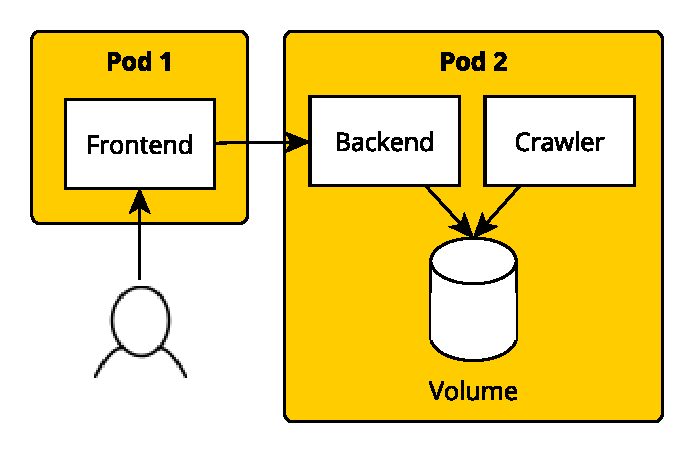
\includegraphics[scale=0.7]{images/figures/pod_example.pdf}
\end{center}
\caption{Example microservice architecture displayed as pods, containers and a volume.}%
\label{fig:pods_example}
\end{figure}

\paragraph{Volumes}%
\label{par:Volumes}

The example in figure~\ref{fig:pods_example} also introduces the concept of
\textit{volumes}. Volumes bring the ability to store files \textit{outside} the
context of the local file system of a container. A pod can specify that it
needs one or more volumes. Each container inside a pod is able to mount these
volumes in the same or a different. The backend from
figure~\ref{fig:pods_example} might mount the volume to
\texttt{/var/www/storage} whereas the crawler wants to mount the volume to
\texttt{/mnt/comics}. Volumes are either local paths on the Kubernetes node or
are maintained by a cloud provider's service like e.g. \textit{Microsoft Azure
File Volumes}.

Simply using the Kubernetes concept of volumes however does pose two significant problems:
\begin{itemize}
  \item For most volume types, the volume has to be provisioned by hand before
    the container can allocate said volume.
  \item The volume is bound to the pods lifecycle. This means that whenever a
    pod is deleted or e.g. dies due to a problem or scaling, the volume needs
    to be recreated during the pod's next startup. This also means that volumes
    can not be defined without first defining a pod.
\end{itemize}

\paragraph{Persistent Volumes, Persistent Volume Claims and Storage Classes}%
\label{par:Persistent_Volume_Claims_and_Storage_Classes}

